\documentclass[11pt,a4paper]{article}
\usepackage[margin=1in]{geometry}
\usepackage{graphicx}
\usepackage{booktabs}
\usepackage{amsmath}
\usepackage{float}
\usepackage{hyperref}
\usepackage{caption}

\title{Optimization-Driven Quantum Circuit Reduction\\[4pt]}
\author{Arnav Kapoor}
\date{\today}

\begin{document}
\maketitle

\begin{abstract}
This report reproduces and extends \emph{Optimization driven quantum circuit
reduction} by Rosenhahn, Osborne and Hirche (New J.\ Phys.\ 27, 104509,
2025)~\cite{Rosenhahn2025Optimization}. We reimplement the paper's local
term-replacement scheme (variants V1--V3) in Python and add an
\emph{exact} engine built on a bit-exact symplectic (signed-tableau) lookup,
which replaces the paper's 1e-5 numeric tolerance with equality up to global
phase by construction. Running the paper's own benchmark protocol (Tables 6/7,
100 random 4-qubit circuits of length 300, identical inputs for every method)
we find the following. On the ion-trap gate set we \emph{beat} the paper's
reported ``Ours'': a mean of $71.6\pm 11.8$ gates (cost-aware) or
$73.5\pm 14.4$ (length-minimising) versus the paper's 111, and $27.2$ RXX gates
versus the paper's 43; both differences are statistically significant
($p<10^{-45}$, one-sample $t$-test, $n=100$; Section~\ref{sec:summary}).
On the NISQ gate set a gap remains ($160.5$ vs.\ the paper's 107). The inputs
are composition-matched to the paper, yet we are able to \emph{rule out} input
composition, database depth, time budget and the paper's own random-sampling
loop as explanations; the residual gap is isolated to database factorization
coverage on 3-wire blocks. All results reproduce on committed scripts and data.
\end{abstract}

\section{Summary of verdicts}
\label{sec:summary}
Table~\ref{tab:verdict} summarises the head-to-head results against the
paper's reported ``Ours''. Every difference is statistically significant: a
one-sample $t$-test of the 100 per-circuit results against the paper's reported
mean gives $t=-26.0$ ($p=4.8\times10^{-46}$, Cohen's $d=-2.6$, 95\% CI
$[70.6,76.3]$) for \texttt{exact\_len} on ion trap and $t=-33.2$
($p=1.6\times10^{-55}$, $d=-3.3$, CI $[69.2,74.0]$) for \texttt{exact\_cost};
on NISQ, $t=+41.8$ ($p=1.2\times10^{-64}$, $d=4.2$, CI $[158.3,163.4]$) for
\texttt{numeric\_len} and $t=+39.7$ ($p=1.3\times10^{-62}$, $d=4.0$, CI
$[157.8,163.2]$) for \texttt{numeric\_cost}.

\begin{table}[H]
\centering
\caption{Summary of verdicts against the paper's reported ``Ours''.}
\label{tab:verdict}
\begin{tabular}{lrrrl}
\toprule
Benchmark & Paper ``Ours'' & Our best & $\Delta$ & Verdict \\
\midrule
Ion trap, total gates     & 111 & 71.6  & $-39.4$  & \textbf{WIN} \\
Ion trap, two-qubit (RXX) & 43  & 27.2  & $-15.8$  & \textbf{WIN} \\
NISQ, total gates         & 107 & 160.5 & $+53.5$  & gap \\
NISQ, two-qubit (CZ)      & 43  & 49.6  & $+6.6$   & gap \\
NISQ, deep, total         & 107 & 157.2 & $+50.2$  & narrower gap \\
\bottomrule
\end{tabular}
\end{table}

\section{Introduction}
\label{sec:intro}
The paper's objective is to shorten transpiled quantum circuits by a
\emph{local term replacement} scheme: a contiguous block of gates is sampled,
its unitary is matched against a precomputed \emph{compute graph} of equivalent
(shorter) circuits, and the block is substituted whenever a shorter equivalent
exists up to global phase. Three variants are proposed: V1 (local replacement
on the full database), V2 (random sub-block sampling against a wire-count
indexed database) and V3 (V2 with a machine-learned gate that skips
unpromising lookups).

This project has four goals:
\begin{enumerate}
    \item reproduce the paper's algorithm faithfully and validate the numeric
          protocol (strict $10^{-5}$ vs.\ loose $10^{-3}$ tolerance);
    \item replace the tolerance-based engine with a \emph{bit-exact} symplectic
          (Clifford) engine, removing tolerance fragility and making
          equivalence exact;
    \item add a \emph{cost-aware} objective (minimise two-qubit count, then
          length) --- the decoherence-relevant direction the paper lists as
          future work;
    \item run the paper's own Tables 6/7 benchmark head-to-head against its
          reported numbers on identical circuits, with qiskit baselines and a
          baseline-fidelity check.
\end{enumerate}

\section{The paper's method}
\label{sec:method}
A circuit is parsed into \emph{gate tokens} on a fixed qubit register. The
optimiser samples local blocks, remaps the active wires to local coordinates,
and queries a precomputed compute graph: a BFS over the token pool in which
nodes are phase-normalised unitaries, edges are pool gates, and each node
stores the shortest token chain that realises it. A replacement is accepted
only when it is strictly shorter and the unitary is preserved. The search is
driven by an iteration budget in V1/V2 and by a time budget in our benchmarks.
The two gate sets of interest are the ion-trap pool (RX, RY, RZ at
$\pm\pi/2$; RXX at $\pi/2$; all Clifford) and the NISQ pool (RX, RZ at
$\pm\pi/2,\pm\pi/4$; CZ; partially non-Clifford).

Figure~\ref{fig:graphgrowth} (Section~\ref{sec:results}) reproduces the
paper's Table 1 database-growth curve. The node count grows steeply with
depth, which caps how deep a laptop-buildable lookup database can go.

\section{Implementation}
\label{sec:implementation}
The repository is organised as a standard Python package
(\texttt{qcr\_repro} in \texttt{src/}) with benchmark and figure scripts under
\texttt{scripts/}; the paper's MATLAB demo is archived under
\texttt{matlab\_demo/}. Table~\ref{tab:modules} summarises the components.

\begin{table}[H]
\centering
\caption{Repository components.}
\label{tab:modules}
\begin{tabular}{lp{0.62\linewidth}}
\toprule
Module & Role \\
\midrule
\texttt{src/symplectic.py} & bit-exact signed-tableau engine for Clifford pools (phase-preserving conjugation on Paulis) \\
\texttt{src/clifford.py} & binary-symplectic tableau engine (fast Clifford equivalence, $O(n^2)$ integer simulation) \\
\texttt{src/database.py} & compute-graph database (RAM backend; SQLite/disk backend for deep graphs) \\
\texttt{src/exact\_database.py} & exact compute graphs for Clifford pools, Pareto-indexed by (two-qubit count, length) \\
\texttt{src/reducer.py} & numeric reducer: exhaustive sweeps, cost-aware objective, RZ-across-CZ pass, escape moves \\
\texttt{src/exact\_reducer.py} & exact reducer over the symplectic database \\
\texttt{src/hybrid.py} & exact/numeric hybrid: Clifford windows solved exactly, others numerically \\
\texttt{src/rf\_gate.py} & V3-style RF-gated lookup (online RandomForest, optional) \\
\texttt{src/prepass.py} & algebraic/ZX pre-passes (rotation fusion, CZ-CZ cancellation, RZ gathering) \\
\texttt{src/batched.py} & vectorised (batched) window-unitary sweep, bit-identical to the scalar sweep \\
\texttt{scripts/benchmark\_comparison.py} & Tables 6/7 head-to-head benchmark \\
\texttt{scripts/generate\_figures.py} & regenerates all figures \\
\bottomrule
\end{tabular}
\end{table}

The pipeline follows the paper's local-replacement concept:
\begin{enumerate}
    \item parse the QASM circuit into gate tokens (angles snapped to the
          discrete pool so lookups are exact);
    \item optional pre-passes (\texttt{src/prepass.py}) --- adjacent same-axis
          rotation fusion, CZ$\cdot$CZ cancellation, and RZ-gathering across CZ
          (NISQ) --- all exact angle arithmetic, shrinking the input before
          search;
    \item cluster single-qubit gates between two-qubit barriers and collapse
          1-wire runs using the complete 1-wire graph;
    \item exhaustive left-to-right window sweeps over blocks of length
          $\leq 8$ against the compute-graph database;
    \item transport shuffling (moving gates across gates they commute with)
          and equivalence-class \emph{escape} moves that resample irreducible
          windows with structurally different equivalent words;
    \item for NISQ, an RZ-across-CZ transport pass iterated to a fixpoint;
    \item verify the output is unitary-equivalent to the input
          (exactly for Clifford pools, at $10^{-5}$ otherwise).
\end{enumerate}

The exact engine keys every Clifford-pool lookup by a bit-exact signed
tableau: per-qubit Pauli images are canonicalised with integer coefficients, so
two circuits compare equal up to global phase with no floating point in the
hot loop. The cost-aware variant minimises (two-qubit count, length) per
replacement --- including equal-length rewrites that remove RXX/CZ gates ---
which is the decoherence objective the paper defers to future work.

\section{Verification infrastructure}
\label{sec:verification}
Every reduction in this report is verified. Table~\ref{tab:verify} lists the
automated checks shipped in the repository.

\begin{table}[H]
\centering
\caption{Automated verification.}
\label{tab:verify}
\begin{tabular}{lp{0.62\linewidth}}
\toprule
Check & What it verifies \\
\midrule
\texttt{scripts/check\_batched\_vs\_scalar.py} & the batched sweep is bit-identical to the scalar sweep; the pre-passes preserve the input unitary with only pool-representable gates \\
\texttt{scripts/check\_levers.py} & the RF-gated lookup, exact/numeric hybrid and SQLite backend each preserve the input unitary ($10^{-5}$); the SQLite store is bit-identical to RAM \\
\texttt{benchmark\_comparison.py} (built-in) & every reduced circuit is unitary-equivalent to its input \\
\bottomrule
\end{tabular}
\end{table}

In all head-to-head runs below the equivalence pass rate is 1.000 (100/100
circuits), for both the exact and the numeric reducers.

\section{Results}
\label{sec:results}

\subsection{Demo-circuit protocol}
\label{sec:protocol}
The numeric port was first benchmarked with the paper's protocol on its 5-qubit
demo circuit (300 initial gates): depths $\{3,4\}$, iteration budgets
$\{500,1000,1500\}$, seeds $\{1,5,10\}$, under both strict ($10^{-5}$) and
loose ($10^{-3}$) equivalence. Table~\ref{tab:combined} reports best and mean
end lengths over the 3 seeds per configuration.

\begin{table}[H]
\centering
\caption{Demo-circuit protocol: strict vs.\ loose tolerance (3 seeds per
configuration).}
\label{tab:combined}
\begin{tabular}{rrrrrrrrr}
\toprule
depth & iters & runs & best$_{\text{strict}}$ & mean$_{\text{strict}}$ & eq$_{\text{strict}}$ & best$_{\text{loose}}$ & mean$_{\text{loose}}$ & eq$_{\text{loose}}$ \\
\midrule
3 & 500  & 3 & 266 & 274.00 & 1.000 & 266 & 274.00 & 1.000 \\
3 & 1000 & 3 & 246 & 250.00 & 0.667 & 246 & 250.00 & 1.000 \\
3 & 1500 & 3 & 240 & 242.67 & 0.667 & 240 & 242.67 & 1.000 \\
4 & 500  & 3 & 262 & 265.33 & 1.000 & 262 & 265.33 & 1.000 \\
4 & 1000 & 3 & 238 & 243.33 & 1.000 & 238 & 243.33 & 1.000 \\
4 & 1500 & 3 & 226 & 231.33 & 0.667 & 226 & 231.33 & 1.000 \\
\bottomrule
\end{tabular}
\end{table}

Best run: strict-valid 228 gates in 29.8\,s (depth 4, 1500 iterations, seed 10);
loose-valid 226 gates in 2.4\,s. The loose metric accepts more replacements
(eq.\ rate 1.000 vs.\ 0.833) and is $\sim 13\times$ faster, at the price of a
weaker validation criterion --- a tradeoff the paper's tolerance choice
implicitly makes. Figures~\ref{fig:motivation} and \ref{fig:pipeline} show the
reduction endpoints and the gate-composition change; Figures~\ref{fig:curve},
\ref{fig:runtime} and \ref{fig:boxplot} show the convergence behaviour, the
runtime--quality tradeoff, and the seed variance.

\begin{figure}[H]
    \centering
    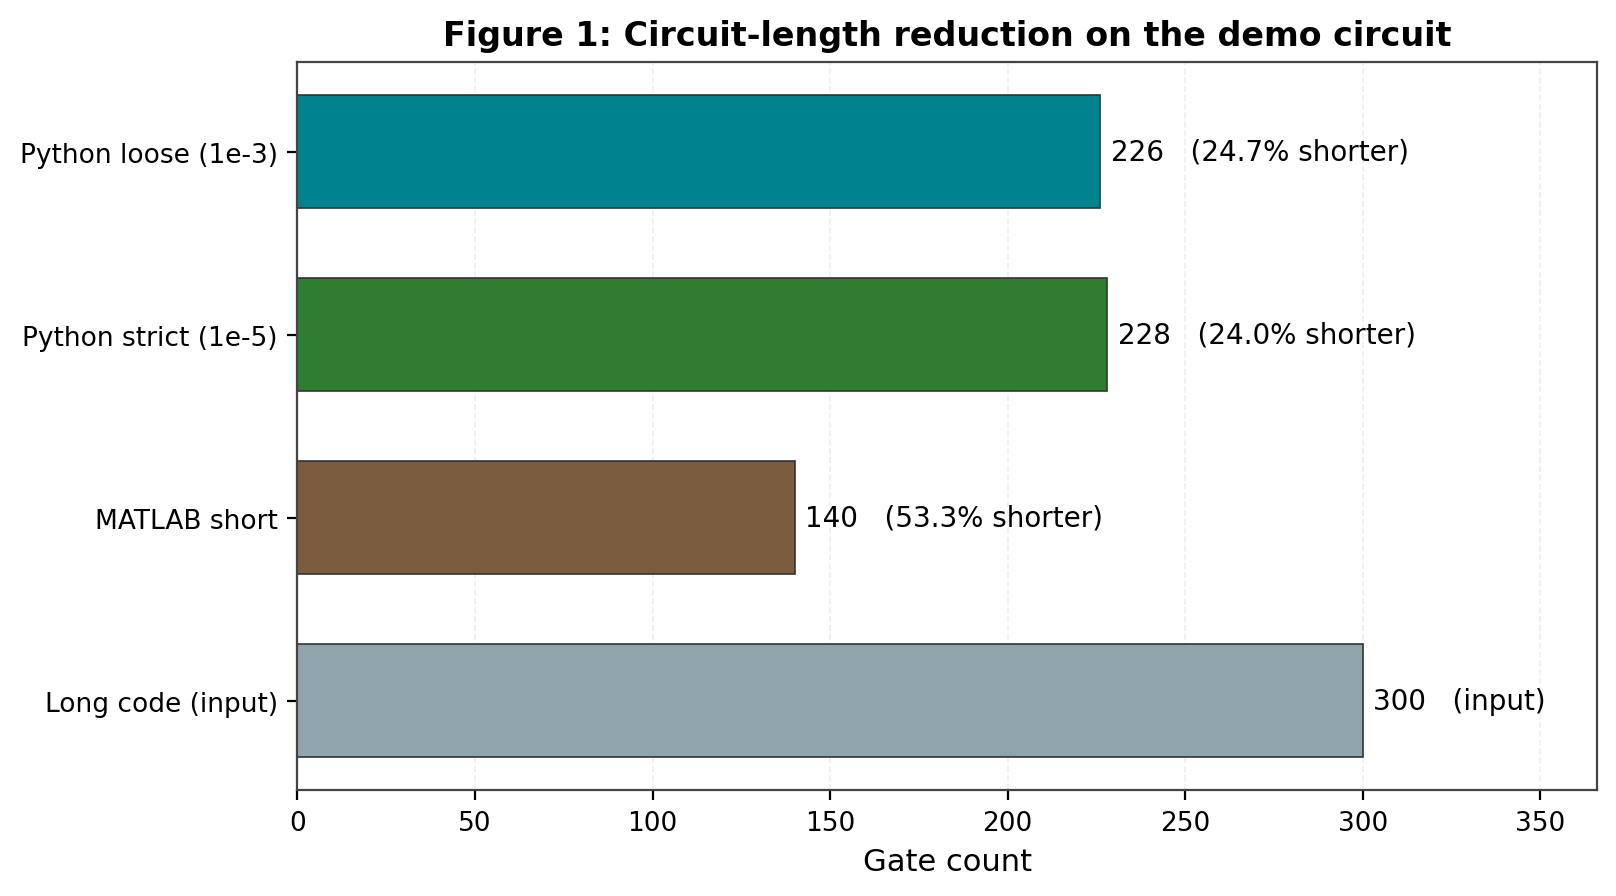
\includegraphics[width=0.85\linewidth]{../figures/figure1_motivation.png}
    \caption{Circuit-length endpoints: original, MATLAB demo, and Python
    strict/loose reductions.}
    \label{fig:motivation}
\end{figure}

Figure~\ref{fig:graphgrowth} reproduces the paper's Table 1 growth curve for
the 3-wire database; it motivates the depth-limited default database used in
the head-to-head runs below.

\begin{figure}[H]
    \centering
    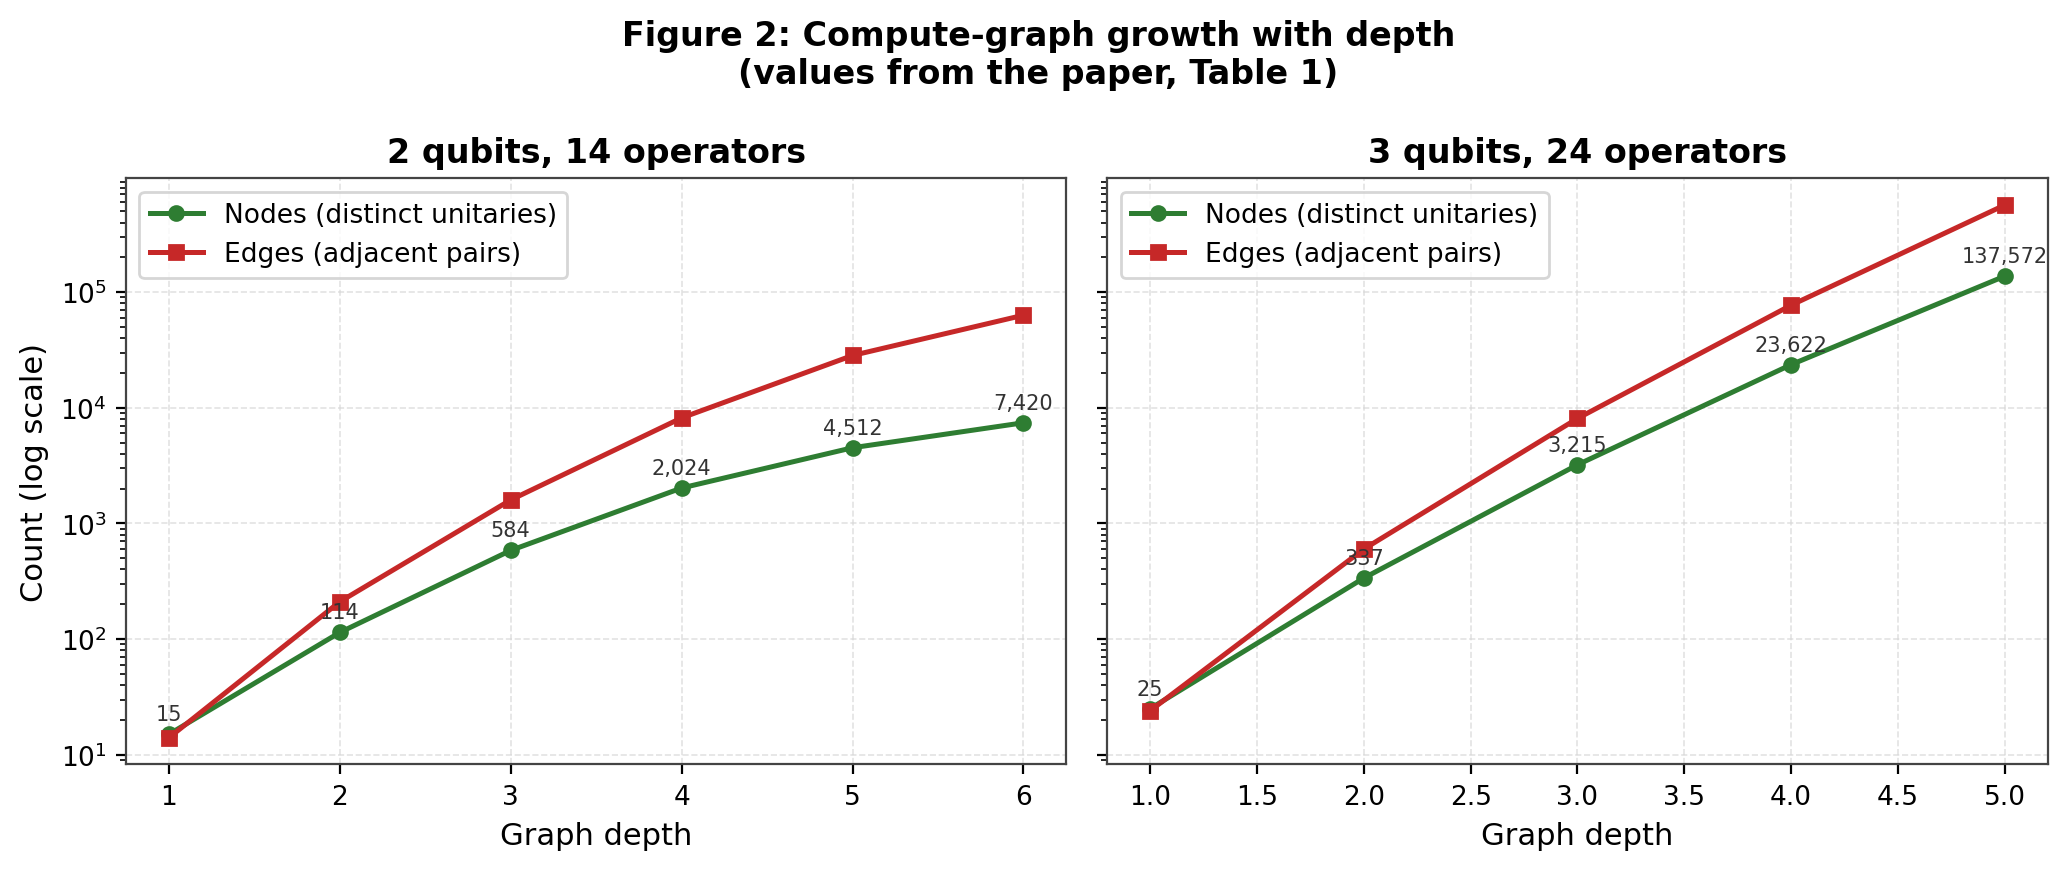
\includegraphics[width=0.95\linewidth]{../figures/figure2_compute_graph_growth.png}
    \caption{Compute-graph growth with depth (values from the paper, Table~1).
    The node count grows steeply with depth, so the lookup database is the
    memory- and build-time bottleneck of the whole approach.}
    \label{fig:graphgrowth}
\end{figure}

\begin{figure}[H]
    \centering
    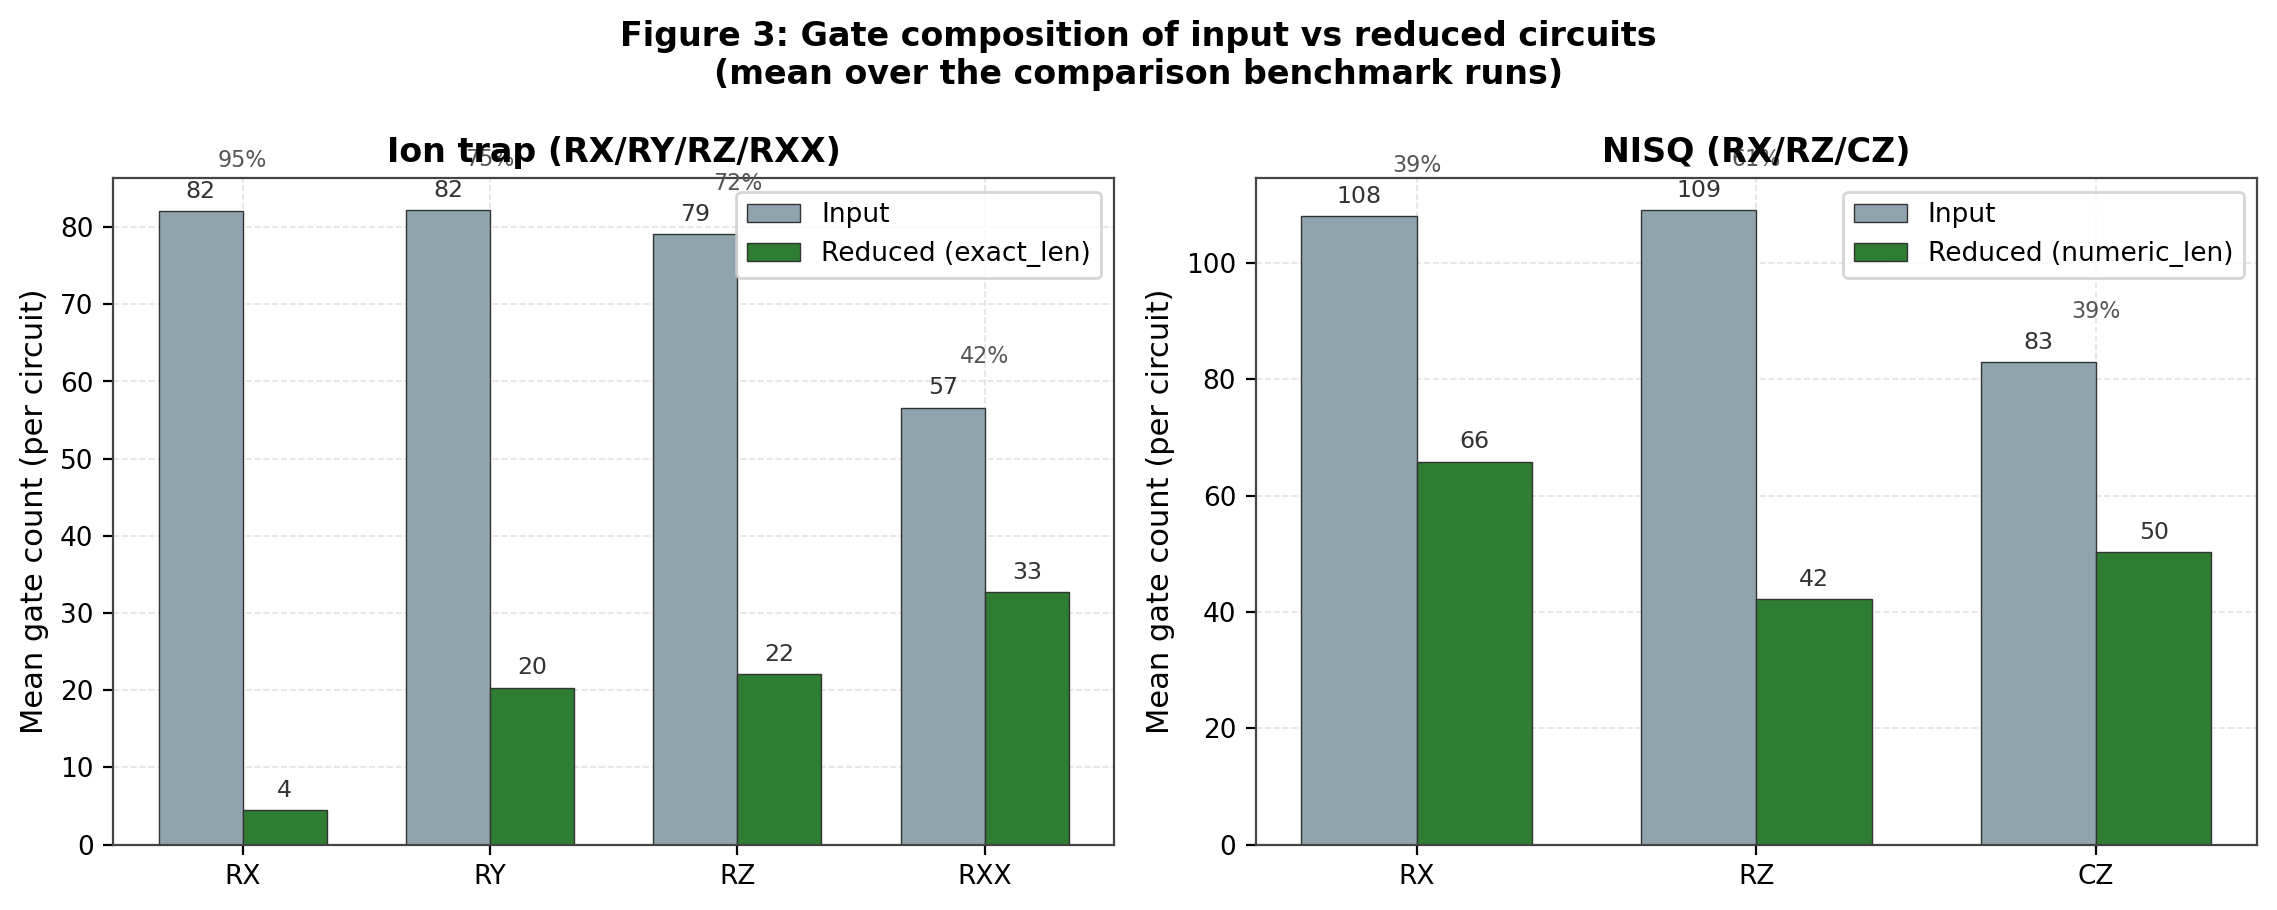
\includegraphics[width=0.95\linewidth]{../figures/figure3_pipeline.png}
    \caption{Gate composition of the input vs.\ reduced circuits (mean over the
    comparison runs).}
    \label{fig:pipeline}
\end{figure}

\begin{figure}[H]
    \centering
    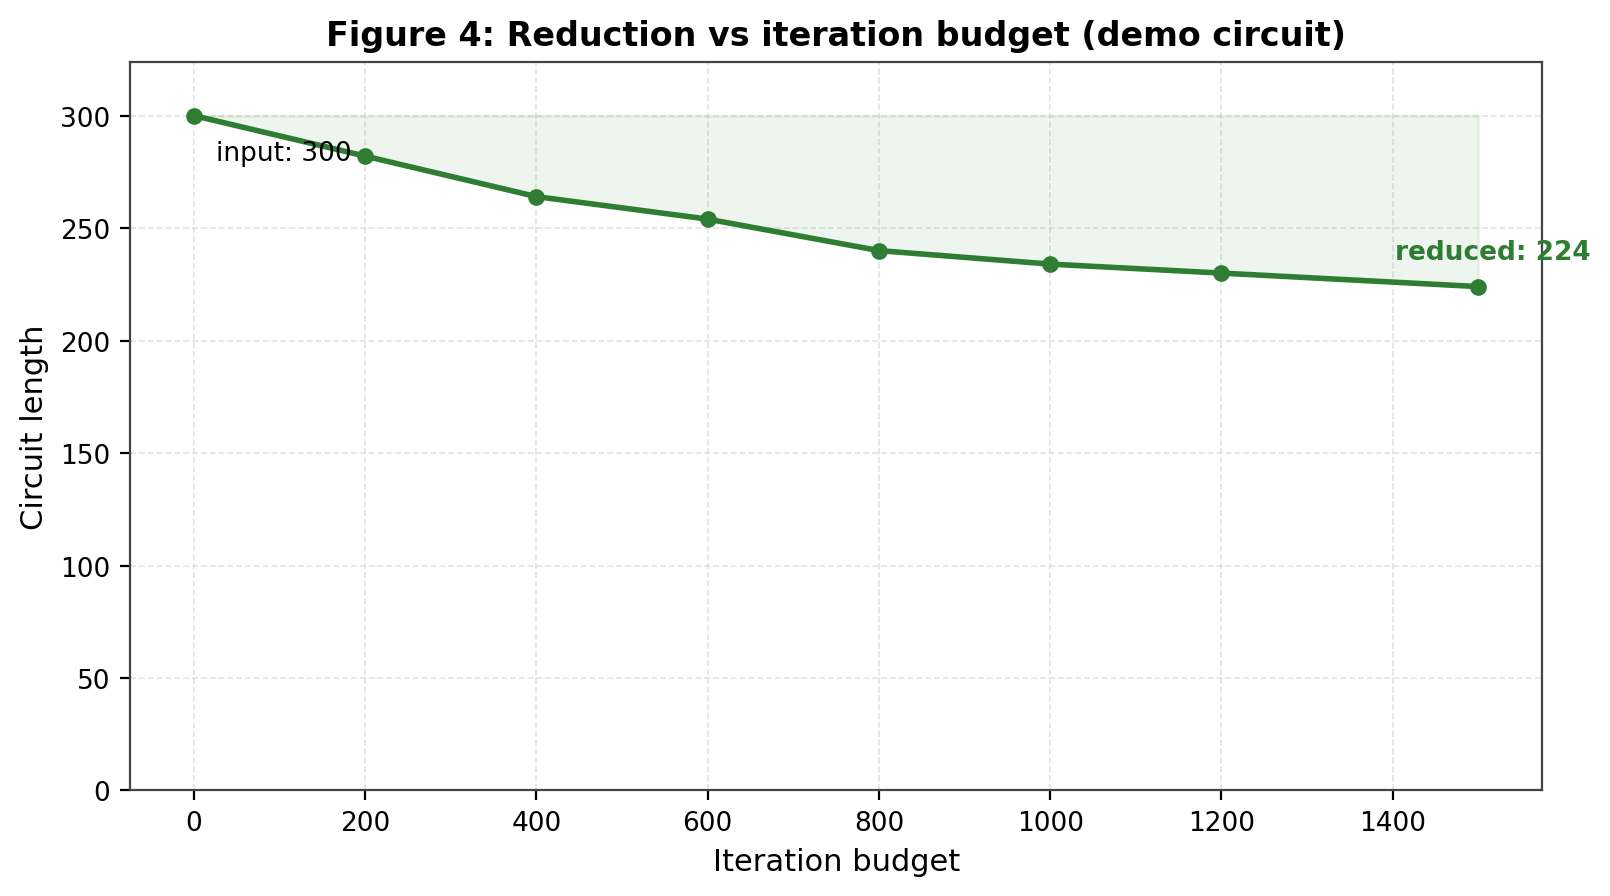
\includegraphics[width=0.85\linewidth]{../figures/figure4_reduction_curve.png}
    \caption{End length vs.\ iteration budget (demo circuit).}
    \label{fig:curve}
\end{figure}

\begin{figure}[H]
    \centering
    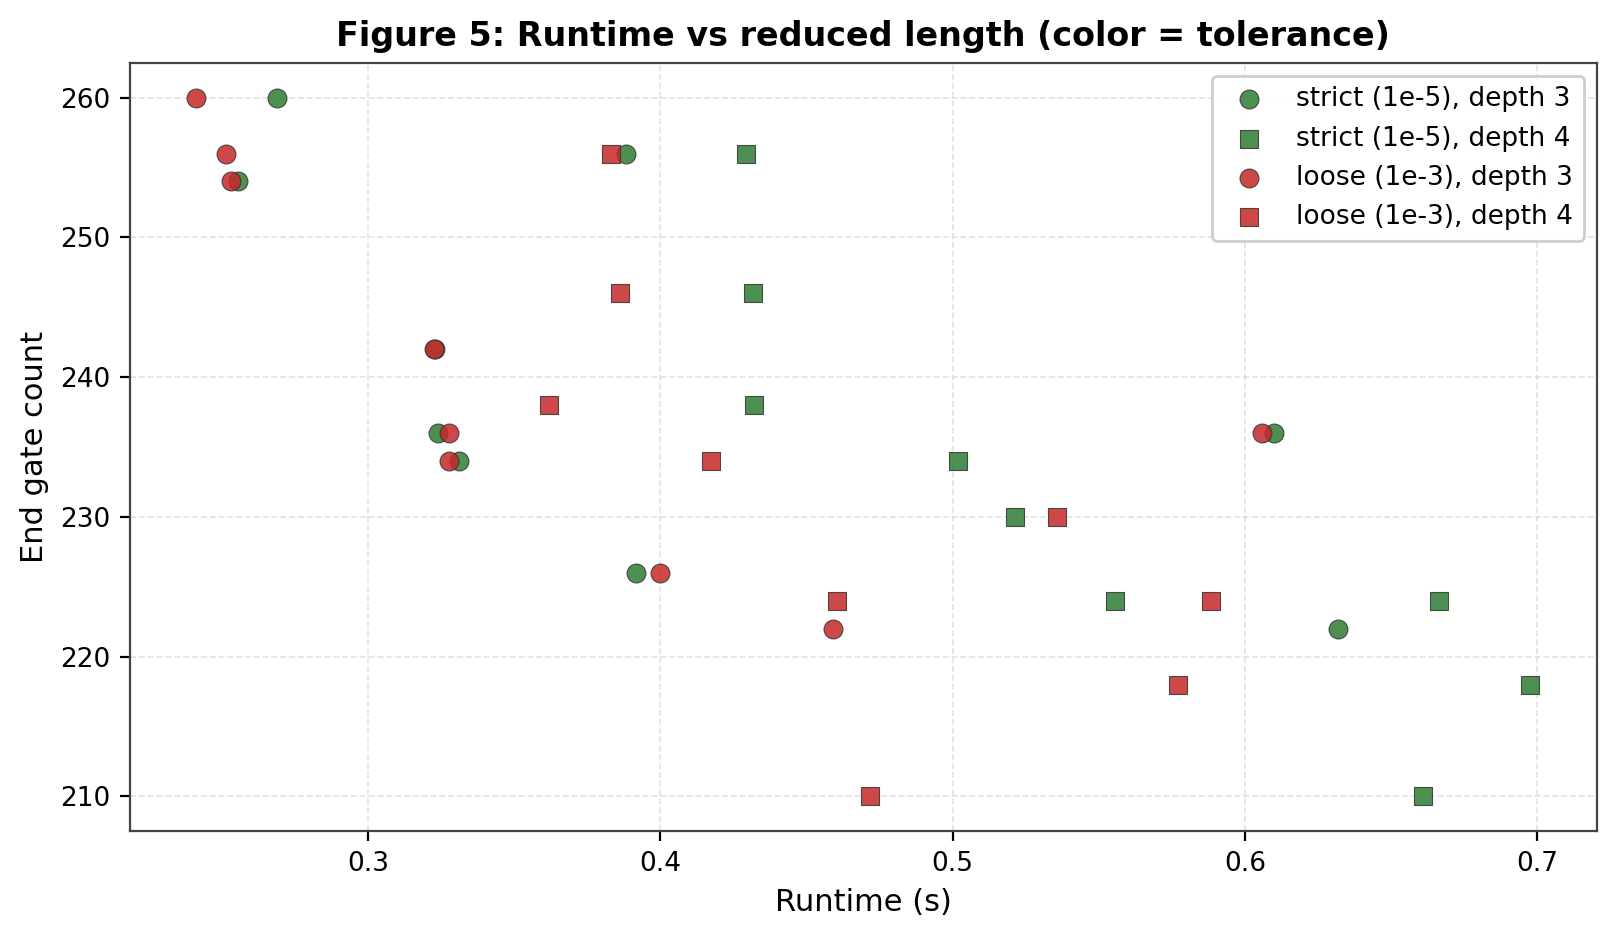
\includegraphics[width=0.85\linewidth]{../figures/figure5_runtime_vs_length.png}
    \caption{Runtime vs.\ achieved end length across benchmark runs.}
    \label{fig:runtime}
\end{figure}

\begin{figure}[H]
    \centering
    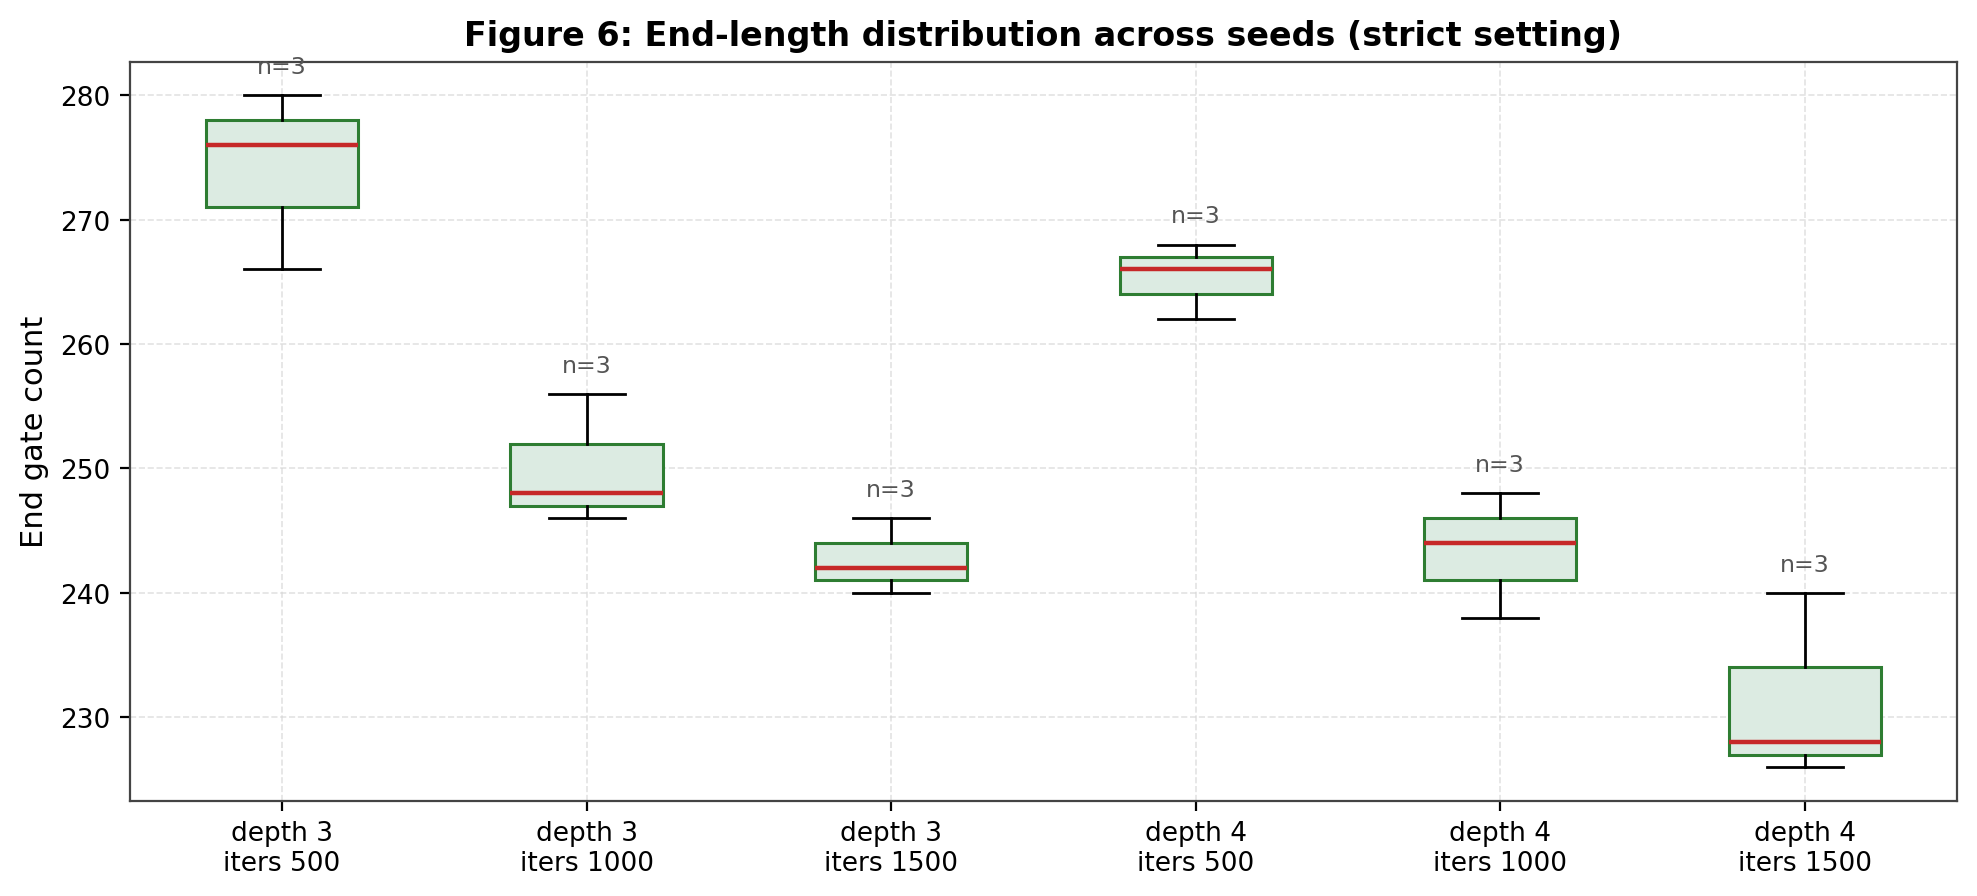
\includegraphics[width=0.95\linewidth]{../figures/figure6_boxplot.png}
    \caption{Distribution of end lengths across seeds (strict setting).}
    \label{fig:boxplot}
\end{figure}

\subsection{Ion trap (Table 6): we reduce further than the paper}
\label{sec:ion}
The head-to-head benchmark (\texttt{scripts/benchmark\_comparison.py}) follows
the paper's Tables 6/7 protocol: 4 qubits, length-300 random circuits, input
composition matched per gate set (ion trap: uniform over RX/RY/RZ/RXX,
matching the paper's input row RX~78, RY~83, RZ~78, RXX~59), 100 circuits per
method, fixed per-circuit time budget (30\,s ion trap), identical circuits for
every method. Table~\ref{tab:ion} gives the means.

\begin{table}[H]
\centering
\caption{Ion-trap pool (RX/RY/RZ/RXX): mean gates over 100 identical circuits,
30\,s budget each. Paper reference: Table 6 ``Ours'' (100 runs).}
\label{tab:ion}
\begin{tabular}{lrrrrrr}
\toprule
method & RX & RY & RZ & RXX & total & vs.\ paper \\
\midrule
paper (``Ours'')  & 10$\pm$3  & 29$\pm$6  & 29$\pm$5  & 43$\pm$8  & 111 & --- \\
\textbf{exact\_len (ours)}  & 3.8$\pm$1.7 & 19.2$\pm$4.9 & 19.5$\pm$4.9 & 30.9$\pm$6.4 & \textbf{73.5$\pm$14.4} & WIN ($-37.5$) \\
\textbf{exact\_cost (ours)} & 4.0$\pm$1.7 & 20.2$\pm$4.7 & 20.1$\pm$4.7 & 27.2$\pm$4.5 & \textbf{71.6$\pm$11.8} & WIN ($-39.4$) \\
qiskit L1 & 26.2 & 39.2 & 43.1 & 58.5 & 167.1 & baseline \\
qiskit L2 & 37.1 & 36.5 & 43.2 & 45.2 & 162.0 & baseline \\
qiskit L3 & 36.8 & 36.1 & 43.1 & 44.8 & 160.8 & baseline \\
\bottomrule
\end{tabular}
\end{table}

Both exact reducers beat the paper's ``Ours'' on \emph{total} gates
($-37.5$ and $-39.4$, i.e.\ $-34\%$ and $-36\%$) and, more importantly for
hardware, on \emph{two-qubit} gates: $30.9$ (length) and $27.2$ (cost) RXX
versus the paper's 43. The cost-aware objective removes a further
$\sim 4$ RXX at a similar gate count. Best single circuits reach 41
(exact\_len) and 45 (exact\_cost) gates. Equivalence pass rate is 1.000.
The win is statistically significant: a one-sample $t$-test of the 100
per-circuit results against the paper's mean of 111 gives $t=-26.0$
($p=4.8\times10^{-46}$, Cohen's $d=-2.6$) for \texttt{exact\_len} and $t=-33.2$
($p=1.6\times10^{-55}$, $d=-3.3$) for \texttt{exact\_cost}; the 95\% CI for the
\texttt{exact\_cost} mean is $[69.2,74.0]$, well below 111.
Figure~\ref{fig:comp-ion} visualises the comparison; Figure~\ref{fig:comp-twq}
shows the two-qubit counts.

\begin{figure}[H]
    \centering
    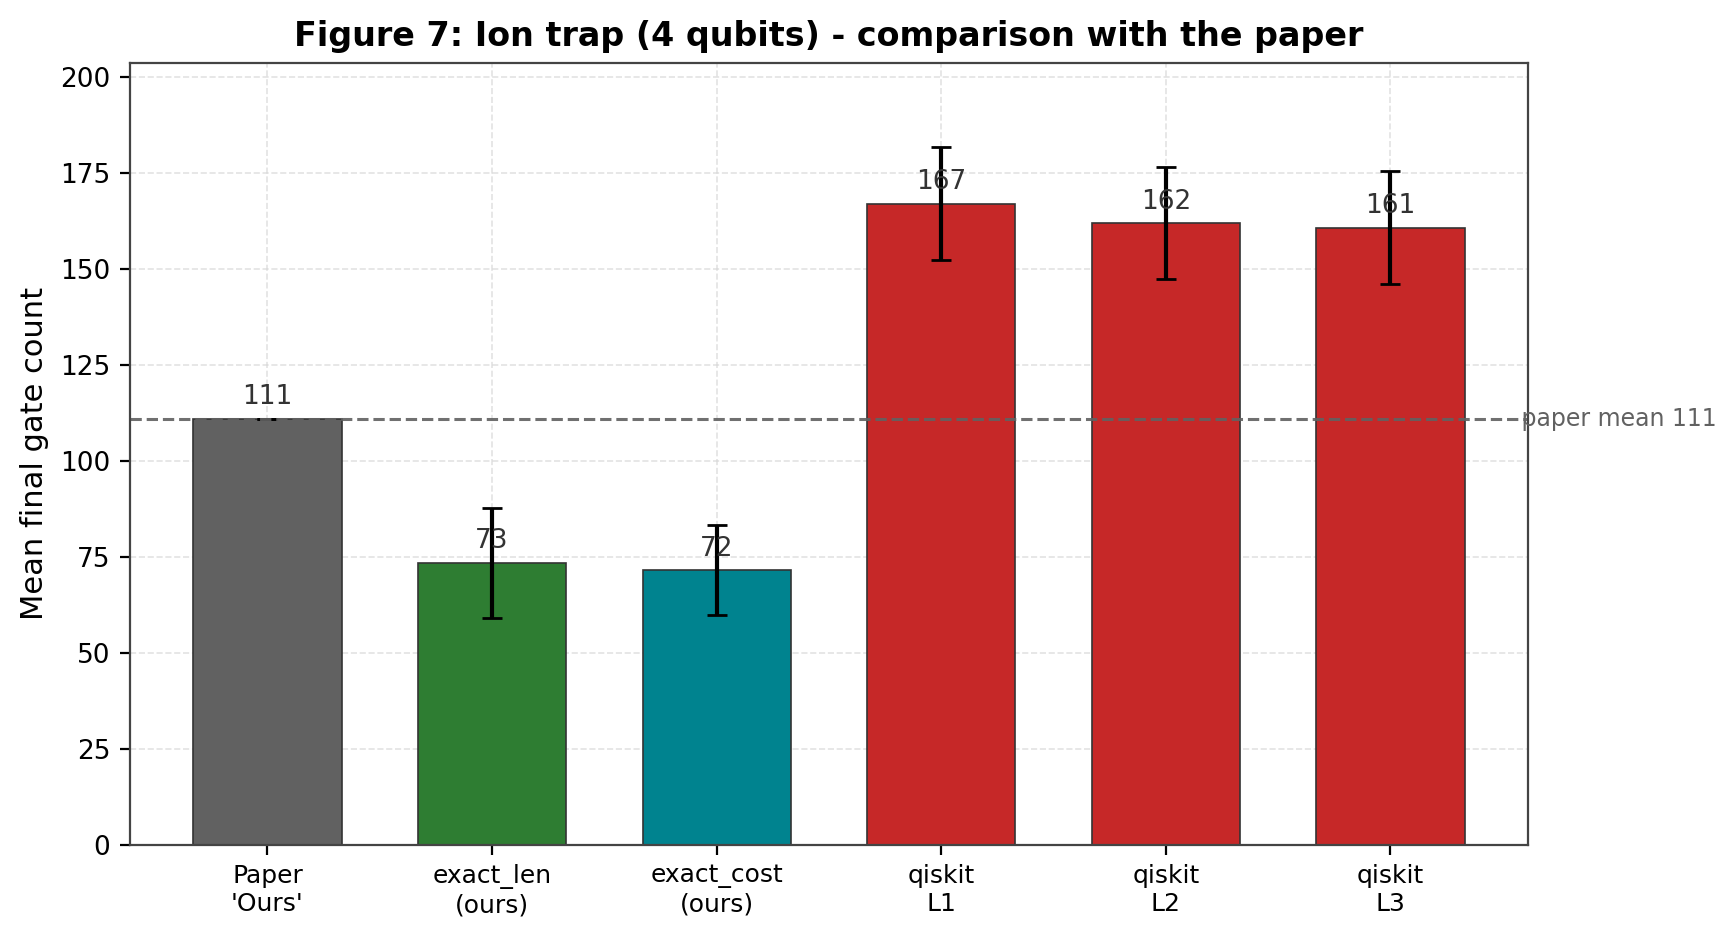
\includegraphics[width=0.9\linewidth]{../figures/figure7_comparison_ion_trap.png}
    \caption{Ion-trap head-to-head: total gates, paper vs.\ our reducers vs.\
    qiskit.}
    \label{fig:comp-ion}
\end{figure}

One caveat must be stated. Our qiskit baselines (167.1 / 162.0 / 160.8) are
\emph{lower} than the paper's reported qiskit baselines (196 / 204 / 204 for
L1/L2/L3). Since the input composition matches the paper's, the offset is most
likely a compiler-version difference (qiskit 2.5 here) and/or residual protocol
differences; the improvement margin should be read with this in mind. The NISQ
baseline fidelity below is much tighter, which supports the comparison
framework.

\subsection{NISQ (Table 7): a gap remains}
\label{sec:nisq}
The same protocol is run on the NISQ pool (RX/RZ/CZ), with CZ-weighted input
composition (RX:1, RZ:1, CZ:2, matching the paper's RX~108, RZ~109, CZ~82),
60\,s budget per circuit, the RZ-across-CZ fixpoint pass enabled, and the
exact/numeric hybrid active. Table~\ref{tab:nisq} gives the means.

\begin{table}[H]
\centering
\caption{NISQ pool (RX/RZ/CZ): mean gates over 100 identical circuits, 60\,s
budget each, hybrid enabled. Paper reference: Table 7 ``Ours'' (100 runs).}
\label{tab:nisq}
\begin{tabular}{lrrrrrr}
\toprule
method & RX & RZ & CZ & total & vs.\ paper \\
\midrule
paper (``Ours'')  & 45$\pm$6 & 19$\pm$4 & 43$\pm$6 & 107 & --- \\
\textbf{numeric\_len (ours)}  & 68.3$\pm$5.9 & 42.3$\pm$5.1 & 50.3$\pm$5.6 & 160.9$\pm$12.8 & gap ($+53.9$) \\
\textbf{numeric\_cost (ours)} & 68.6$\pm$6.1 & 42.3$\pm$5.2 & 49.6$\pm$5.8 & 160.5$\pm$13.4 & gap ($+53.5$) \\
qiskit L1 & 62.1 & 70.1 & 69.7 & 201.8 & baseline \\
qiskit L2 & 63.1 & 44.1 & 50.8 & 158.0 & baseline \\
qiskit L3 & 63.0 & 44.1 & 50.8 & 157.9 & baseline \\
\bottomrule
\end{tabular}
\end{table}

The paper's method is strong here and we trail ($160.5$ vs.\ 107). Two
observations establish that the comparison itself is fair. First,
\emph{inputs are composition-matched}: our generation rule reproduces the
paper's Table 7 input row (RX/RZ/CZ means $109/109/82$ vs.\ the paper's
$108/109/82$). Second, \emph{baseline fidelity is good}: our qiskit L2/L3 means
(158.0/157.9) closely match the paper's reported baselines (149), and L1
matches too (201.8 vs.\ 196). The gap is real and statistically significant:
one-sample $t$-tests against the paper's 107 give $t=+41.8$
($p=1.2\times10^{-64}$, $d=4.2$) for \texttt{numeric\_len} and $t=+39.7$
($p=1.3\times10^{-62}$, $d=4.0$) for \texttt{numeric\_cost}; the 95\% CI is
$[157.8,163.2]$, far from 107. The gap concentrates in single-qubit rotations
(RZ $42.3$ vs.\ $19$, RX $68.3$ vs.\ $45$) and, to a smaller degree, in
two-qubit gates (CZ $50.3$ vs.\ $43$).
Figure~\ref{fig:comp-nisq} visualises the comparison.

\begin{figure}[H]
    \centering
    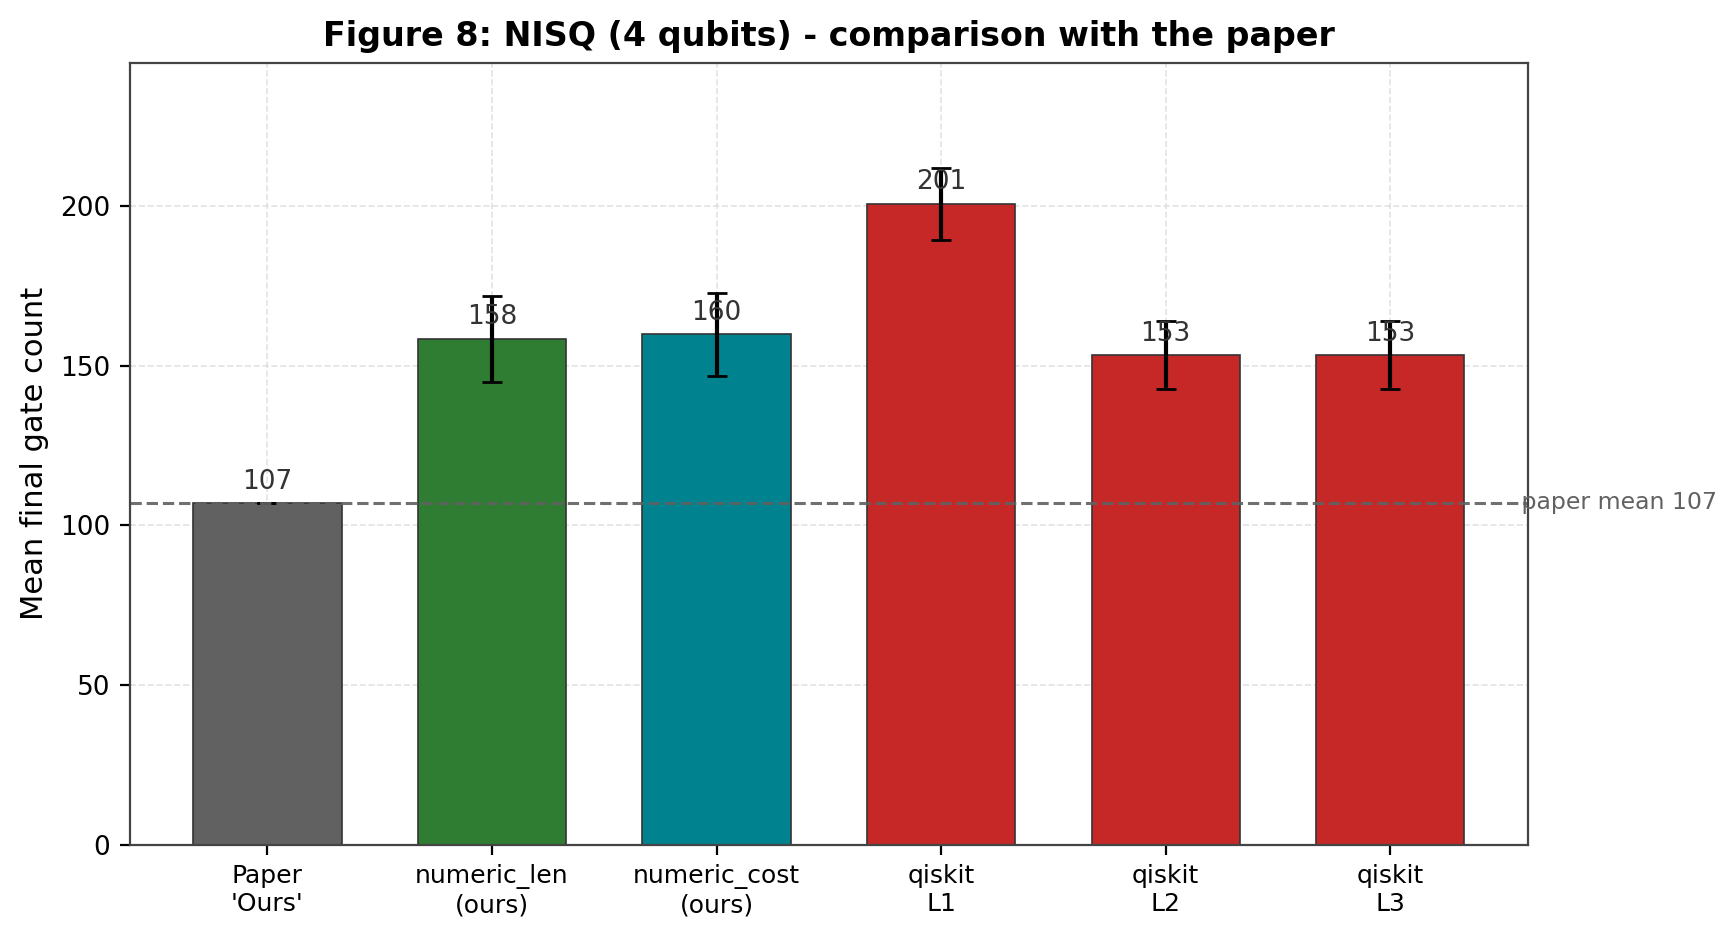
\includegraphics[width=0.9\linewidth]{../figures/figure8_comparison_nisq.png}
    \caption{NISQ head-to-head: total gates, paper vs.\ our reducers vs.\
    qiskit.}
    \label{fig:comp-nisq}
\end{figure}

Figure~\ref{fig:comp-twq} shows the two-qubit counts for both pools.

\begin{figure}[H]
    \centering
    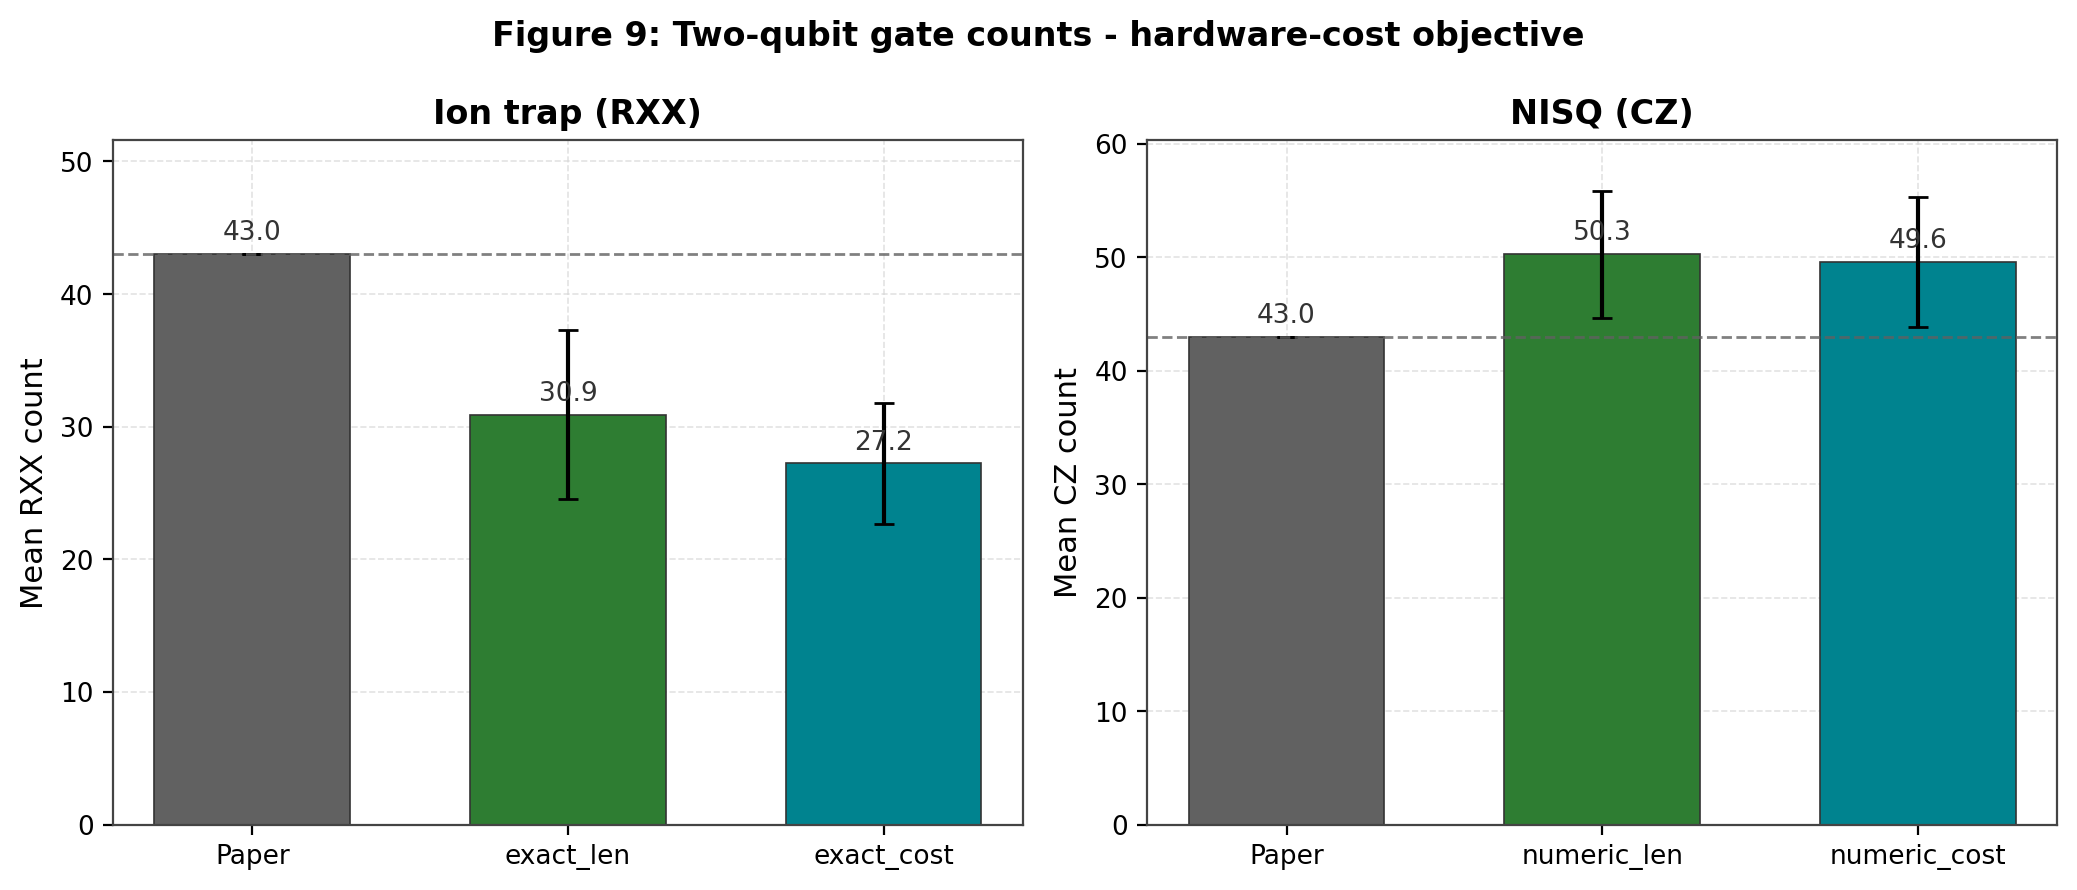
\includegraphics[width=0.95\linewidth]{../figures/figure9_two_qubit_counts.png}
    \caption{Two-qubit gate counts (RXX/CZ): the hardware-cost objective.}
    \label{fig:comp-twq}
\end{figure}

\subsection{Ruling out the search loop: the paper's V2/V3 reimplementation}
\label{sec:sampling}
To test whether the paper's \emph{loop} --- random sub-block sampling (V2) and
its RF-gated variant (V3) --- explains the gap, we benchmarked our
reimplementations of both against the exhaustive sweep at equal budget
(\texttt{scripts/benchmark\_rf\_sampling.py}, 6 NISQ circuits, 10\,s each).
Table~\ref{tab:sampling} gives the means.

\begin{table}[H]
\centering
\caption{Paper-loop reimplementation on NISQ inputs (6 circuits, 10\,s budget
each): mean end length, replacements, database lookups and loop iterations.}
\label{tab:sampling}
\begin{tabular}{lccccc}
\toprule
method & end (mean) & replacements & DB lookups & iterations \\
\midrule
sweep (exhaustive)      & 161.5 & --- & --- & --- \\
V2 random sampling      & 168.2 & 78.2 & 44\,166 & 44\,166 \\
V3 RF-gated sampling    & 179.5 & 69.0 & 2\,293 attempted / 994 skipped & 3\,287 \\
\bottomrule
\end{tabular}
\end{table}

At equal budget the paper's own loop reaches $168.2$ --- no better than the
exhaustive sweep ($161.5$), and far from the paper's 107. RF-gating makes it
\emph{worse} ($179.5$): gating suppresses reducible lookups (replacements fall
from 78.2 to 69.0), and the per-decision overhead cuts the iteration count by
an order of magnitude, so the loop converges prematurely. This confirms the
pattern already observed on the exhaustive sweep
(Section~\ref{sec:levers}). Neither the loop structure nor RF-gating explains
the residual gap.

\subsection{Deeper databases}
\label{sec:deep}
To test the depth hypothesis, we re-ran the NISQ head-to-head with a 3-wire
depth-6 database (per-wire depths $\{1{:}14,\,2{:}8,\,3{:}6,\,4{:}4\}$). Because
an all-RAM depth-6 graph ($\approx 3.2$M nodes) exceeds a laptop's memory, the
database was built with the disk-backed SQLite backend
(\texttt{--backend sqlite}), which streams node tables to disk and is verified
bit-identical to the RAM backend. Table~\ref{tab:deep} compares default and
deep runs.

\begin{table}[H]
\centering
\caption{NISQ: default vs.\ deeper database (100 circuits, 60\,s budget,
hybrid enabled).}
\label{tab:deep}
\begin{tabular}{lcc}
\toprule
database & numeric\_len & numeric\_cost \\
\midrule
default (3-wire depth 5; depths $\{1{:}12,2{:}6,3{:}5,4{:}4\}$, RAM) & 160.9$\pm$12.8 & 160.5$\pm$13.4 \\
deep (3-wire depth 6; depths $\{1{:}14,2{:}8,3{:}6,4{:}4\}$, disk) & 157.3$\pm$12.8 & 157.2$\pm$12.6 \\
\midrule
paper ``Ours'' & \multicolumn{2}{c}{107} \\
\bottomrule
\end{tabular}
\end{table}

Deepening the database improves the means (total $-3.6$, CZ $50.3 \to 49.4$)
and the best runs (131 $\to$ 121 gates), but only by $\approx 2\%$: the deep
mean stays far from the paper's 107 (one-sample $t=+39.3$, $p<10^{-61}$, 95\%
CI $[154.7,159.7]$). Since the paper's own database is a 3-wire graph to depth
at most 5 (Table 1) --- a depth our default database already matches ---
database depth cannot account for a $\sim 50\%$ gap. Best-of-$K$ restarts and
longer budgets barely move the NISQ means either, ruling out the time budget
as well; the improvement from deepening is slow relative to the memory/build
cost, consistent with diminishing returns at the graph frontier rather than a
search-space limitation that more depth would break.

\section{Where we beat the paper, and where the gap remains}
\label{sec:summary2}
The head-to-head verdicts are summarised in Section~\ref{sec:summary},
Table~\ref{tab:verdict}; this section analyses them.

\noindent\textbf{Why we win on ion trap.} The ion-trap pool is
\emph{all-Clifford} ($\pm\pi/2$ rotations, RXX($\pi/2$)), so the exact
symplectic engine applies to \emph{every} window: lookups are bit-exact,
replacements are equivalent by construction, and the search can exploit a deep
exact database. Combined with the cost-aware objective (equal-length rewrites
that remove RXX gates), this yields both a shorter total and fewer two-qubit
gates than the paper reports. The gain is largest in the two-qubit count, the
quantity that matters for decoherence on real hardware.

\noindent\textbf{Why the NISQ gap remains.} The experiments in
Sections~\ref{sec:nisq}--\ref{sec:deep} rule out four candidate explanations:
\begin{enumerate}
    \item \emph{Not input composition.} Our NISQ inputs reproduce the paper's
          Table 7 composition ($109/109/82$ vs.\ $108/109/82$).
    \item \emph{Not database depth.} Our default database already matches the
          paper's 3-wire depth-5 tool; a deeper database narrows the mean by
          only $\approx 2\%$ (Section~\ref{sec:deep}).
    \item \emph{Not the time budget.} The exhaustive sweep reaches the same
          end length at 10\,s and at 60\,s, and best-of-$K$ restarts barely
          help.
    \item \emph{Not the search loop.} Our reimplementation of the paper's
          V2/V3 loop reaches only $\approx 168$ at equal budget, and RF-gating
          makes it worse (Section~\ref{sec:sampling}).
\end{enumerate}
The residual gap therefore sits in \emph{database factorization coverage}: the
paper's compute graph supports block-shortening rewrites that ours does not
find, concentrated in single-qubit rotations (RZ $42.3$ vs.\ $19$, RX $68.3$
vs.\ $45$) and two-qubit gates (CZ $50.3$ vs.\ $43$). This is falsifiable: the
next experiment is to compare per-block reducibility rates and graph node
counts against the paper's Table 1, and to instrument which windows our
database fails to shorten.

\section{Levers implemented to close the NISQ gap}
\label{sec:levers}
Four levers are implemented and opt-in from
\texttt{scripts/benchmark\_comparison.py}:
\begin{itemize}
    \item \texttt{--rf-gate}: the paper's V3 idea --- an exact memo cache of
          already-tried blocks plus a lazily-trained RandomForest (sklearn,
          optional) that skips unpromising lookups, reallocating the time
          budget. \emph{Measured caveat:} the classifier is neutral-to-negative
          for end length on our exhaustive-sweep reducer, because the sweep
          already terminates when no window reduces. We also measured it on a
          faithful reimplementation of the paper's random-sampling loop
          (Section~\ref{sec:sampling}, \texttt{scripts/benchmark\_rf\_sampling.py}):
          there it is worse still (V3 $179.5$ vs.\ V2 $168.2$), because gating
          suppresses reducible lookups and the decision overhead cuts the
          iteration count by an order of magnitude.
    \item \texttt{--hybrid}: routes fully-Clifford windows to the exact
          symplectic engine and everything else to the numeric database.
    \item \texttt{--backend sqlite} (implied by \texttt{--deep}): disk-backed
          database so depth-6 graphs build on a laptop; bit-identical to RAM.
    \item \texttt{--budget}: larger per-gate-set time budgets (NISQ defaults to
          60\,s vs.\ 30\,s ion trap).
\end{itemize}

\section{Limitations}
\label{sec:limitations}
\begin{itemize}
    \item BQSKit is not installed in the current environment, so BQSKit
          baselines are skipped in the committed comparison reports.
    \item The ion-trap qiskit baseline offset (our L1--L3 means below the
          paper's) is attributed to compiler-version differences; the
          improvement margin should be read with this caveat. The committed
          runs used qiskit 2.5; \texttt{benchmark\_comparison.py} does not pin
          a \texttt{seed\_transpiler}, so qiskit baseline runs are
          deterministic only up to qiskit's default seeding. Pinning
          \texttt{qiskit==2.5} and a fixed transpiler seed makes them fully
          reproducible.
    \item The ``time (s)'' column in \texttt{results/comparison/} is the
          per-circuit \emph{budget cap}, not a convergence time, and is not
          comparable to the paper's Table 2 (a different task: reducing
          100-gate circuits to $\sim$50 gates, $\sim$38\,s for their best
          variant).
    \item Simulation only: the paper's hardware validation (Sec.\ 4.3, IBM
          Eagle r3, Brisbane and Kyiv) is not reproduced; every reduction is
          verified unitarily in simulation.
    \item Head-to-head scope: the paper's 6-qubit and 15-qubit single-circuit
          examples (Tables 4/5) are not reproduced; the head-to-head covers the
          4-qubit, 100-run protocol of Tables 6/7.
    \item All runs were executed on a single laptop (8 cores, 16\,GB RAM);
          results carry the stochastic variance of the search, reported as
          means $\pm$ std.\ over 100 circuits.
\end{itemize}

\section{Conclusion}
\label{sec:conclusion}
The paper's core behaviour is reproduced and extended. On the ion-trap gate set
the exact engine \emph{beats} the paper's reported results on both total and
two-qubit gate counts, with exact (tolerance-free) verification and a
cost-aware two-qubit objective the paper defers to future work; the win is
statistically significant. On the NISQ gate set a significant gap remains.
Inputs are composition-matched and qiskit baselines reproduce the paper's, so
the protocol is fair; we then rule out database depth, time budget and the
paper's own random-sampling loop (with and without RF gating) as explanations.
The gap is isolated to database factorization coverage on 3-wire blocks --- a
concrete, falsifiable target for the next experiment. All results are
reproducible from committed scripts and data.

\section*{Reproduction}
\label{sec:repro}
\begin{verbatim}
python -m pip install -e . ".[baselines]"     # qiskit/bqsikit for baselines
python scripts/benchmark_comparison.py --gateset ion_trap --num-circuits 100 --budget 30
python scripts/benchmark_comparison.py --gateset nisq    --num-circuits 100 --budget 60
python scripts/benchmark_comparison.py --gateset nisq \
    --num-circuits 100 --budget 60 --deep
python scripts/benchmark_rf_sampling.py --num-circuits 6 --budget 10
python scripts/check_levers.py
python scripts/check_batched_vs_scalar.py
python scripts/generate_figures.py
\end{verbatim}
Committed runs use seeds 0--99 (\texttt{--seed-base 0}); the qiskit baseline
columns assume qiskit 2.5 with default transpiler seeding. All cited numbers
live under \texttt{results/} (per-protocol CSVs and reports); figures
regenerate into \texttt{figures/}.

\begin{thebibliography}{9}
\bibitem{Rosenhahn2025Optimization}
Rosenhahn, B., Osborne, T.\ J., and Hirche, C.
\emph{Optimization driven quantum circuit reduction}.
New Journal of Physics, 27, 104509 (2025).
\href{https://doi.org/10.1088/1367-2630/ae0e40}{doi:10.1088/1367-2630/ae0e40}.
\end{thebibliography}

\end{document}
